\documentclass[12pt]{article}
\usepackage{geometry}                % See geometry.pdf to learn the layout options. There are lots.
\geometry{letterpaper}                   % ... or a4paper or a5paper or ... 
%\geometry{landscape}                % Activate for for rotated page geometry
\usepackage[parfill]{parskip}    % Activate to begin paragraphs with an empty line rather than an indent
\usepackage{daves,fancyhdr,natbib,graphicx,dcolumn,amsmath,lastpage,url}
\usepackage{amsmath,amssymb,epstopdf,longtable}
\usepackage[final]{pdfpages}
\DeclareGraphicsRule{.tif}{png}{.png}{`convert #1 `dirname #1`/`basename #1 .tif`.png}
\pagestyle{fancy}
\lhead{CE 3105 Fluid Mechanics (CECE) Laboratory}
\rhead{FALL 2025}
\lfoot{}
\cfoot{}
\rfoot{Page \thepage\ of \pageref{LastPage}}
\renewcommand\headrulewidth{0pt}



\begin{document}
\begin{centering}
\textbf{CE 3105 Laboratory Report}\\
P. Olar Bear - Team 1\\
2025-0825\\
CE 3105 Fluid Mechanics Laboratory\\
Lab X\\
\textbf{Calibration of a Pitot Tube Using a Wind Tunnel}\\
TA: P. N. Guinn\\
Monday/09:00\\
\end{centering}
\clearpage

\section{Calibration of a Pitot Tube Using a Wind Tunnel}

Objective: The objective of this experiment is to calibrate a Pitot tube by measuring the dynamic pressure in a wind tunnel at varying airspeeds. The experiment will compare the velocity determined by the Pitot tube to the known airspeed from the wind tunnel and provide a calibration curve for the Pitot tube.\footnote{This example provides a generic outline. Adapt your report to reflect the specific equipment and procedures available in your lab.
Pay careful attention to environmental conditions as they significantly affect fluid density and, consequently, your results. Some laboratory experiments will have substantially more complex data collection steps.} \\

\section{Background/Theory:}
A Pitot tube measures the velocity of a fluid (in this case, air) by comparing the total pressure at the stagnation point with the static pressure in the flow. The difference between these pressures, known as the dynamic pressure, is used to calculate the airspeed using Bernoulli’s equation:

\begin{equation}
V=\sqrt{2 \times \frac{\Delta P}{\rho}}
\end{equation}

where:

    $V$ is the airspeed (m/s),\\
    $\Delta P$ is the difference between total and static pressures (Pa),\\
    $\rho$ is the air density ($kg/m^3$).\\

The purpose of this experiment is to calibrate the Pitot tube by comparing the measured airspeed (using the Pitot tube and Bernoulli’s equation) to the actual airspeed set by the wind tunnel.
%%%%%%%%%%%%%%%%%%%%%%%%%%%%
\clearpage

\section{Materials and Equipment:} 
\begin{itemize}
\item Pitot tube
\item Wind tunnel (with variable airspeed control)
\item Differential pressure transducer
\item Data acquisition system (DAQ) connected to pressure transducer
\item Barometer (to measure atmospheric pressure)
\item Thermometer (to measure ambient air temperature)
\item Calculator or software for data analysis
\item Safety goggles
\end{itemize}
%%%%%%%%%%%%%%%%%%%%%%%%%%%%
\clearpage

\section{Experimental Setup:}
\begin{enumerate}
\item Wind Tunnel Setup:

Securely mount the Pitot tube in the test section of the wind tunnel, ensuring that the tube’s tip is aligned with the airflow direction. 
The Pitot tube should be positioned at the center of the airflow to avoid boundary layer effects.

\item Pressure Measurement System:

Connect the Pitot tube to the differential pressure transducer. 
Ensure that the total pressure tap (stagnation pressure) is connected to the positive side of the transducer and the static pressure tap to the negative side.

\item Data Acquisition:

Connect the pressure transducer to the data acquisition system (DAQ). Calibrate the DAQ system according to the manufacturer’s specifications to ensure accurate pressure readings. The DAQ will record the pressure difference, $\Delta P$, at various wind speeds.

\item Environmental Conditions:

Measure the ambient air temperature and barometric pressure to calculate air density, $\rho$. Use the following equation to compute air density:
\begin{equation}
\rho=\frac{P}{R \cdot T}
\end{equation}
where:
\begin{itemize}
\item $P$ is the atmospheric pressure ($Pa$),
\item $R$ is the specific gas constant for dry air ($287~\frac{J}{kg} \cdot K$), and
\item $T$ is the absolute temperature ($K$).
\end{itemize}
\end{enumerate}
%%%%%%%%%%%%%%%%%%%%%%%%
\clearpage

\section{Procedure:} 
\begin{enumerate}
\item Start the Wind Tunnel:
\begin{itemize}
\item Turn on the wind tunnel and set it to the lowest airspeed (e.g., 5 m/s).
\item Record the differential pressure, $\Delta P$, using the DAQ system.
\item Note the wind tunnel’s airspeed from its control system as the reference velocity.
\end{itemize}
\item Increase the Wind Speed:
\begin{itemize}
\item Gradually increase the airspeed of the wind tunnel in increments (e.g., 5 m/s increments) up to the maximum speed of the wind tunnel.
\item For each speed increment, record the differential pressure, $\Delta P$, from the DAQ system.
\end{itemize}
\item Repeat Measurements:
\begin{itemize}
\item At each airspeed, take at least three readings of $\Delta P$ to ensure consistency and accuracy. Compute the average $\Delta P$ for each airspeed.
\end{itemize}
\item Shutdown:
\begin{itemize}
\item After collecting data for all airspeeds, shut down the wind tunnel and disconnect the Pitot tube from the system.
\end{itemize}
\end{enumerate}
%%%%%%%%%%%%%%%%%%%%%%%%%%%%%
\clearpage

\section{Data Collection:} 

Collect $\Delta P$ at $5~m/s$ speed increments to populate a data table similar to Table \ref{tab:datatable} below. \footnote{Your data should be for every measurement, so there will be at least 3 measurements per windspeed. Perfom the indicated avaerging in the data analysis section of the report!}
\begin{table}[h!]
\centering
\caption{Wind Tunnel Settings and Pitot Tube Pressure Drop}
\begin{tabular}{p{1.5in}p{1.5in}p{1.5in}}
~&~&~\\
Wind Tunnel Airspeed (m/s)&Measured $\Delta P$ (Pa)&Calculated Airspeed (m/s)\\
\hline
\hline
5&15&4.87\\
10&60&9.75\\
15&135&14.61\\
20&240&19.48\\
25&375&24.35\\
\hline
\end{tabular}
\label{tab:datatable}
\end{table}
%%%%%%%%%%%%%%%%%%%%%%%%%%%%%
\clearpage

\section{Data Analysis:}
\begin{enumerate}

\item Calculate the Airspeed:
Use the measured $\Delta P$ values and the air density, $\rho$, to compute the airspeed using Bernoulli’s equation:

\begin{math}
V=\sqrt{2 \times \frac{\Delta P}{\rho}}
\end{math}

Example calculation: For $\Delta P =15~Pa$, assuming $\rho=1.225~kg/m^3$:\\

\begin{math}
V=\sqrt{2\times \frac{\Delta P}{\rho}}
V=\sqrt{2} \times \sqrt{\frac{15}{1.225}} = 4.87~m/s \\
\end{math}


\end{enumerate}
%%%%%%%%%%%%%%%%%%%%%%%%%%%%%
\clearpage

\section{Results}

\begin{figure}[h!] %  figure placement: here, top, bottom, or page
   \centering
   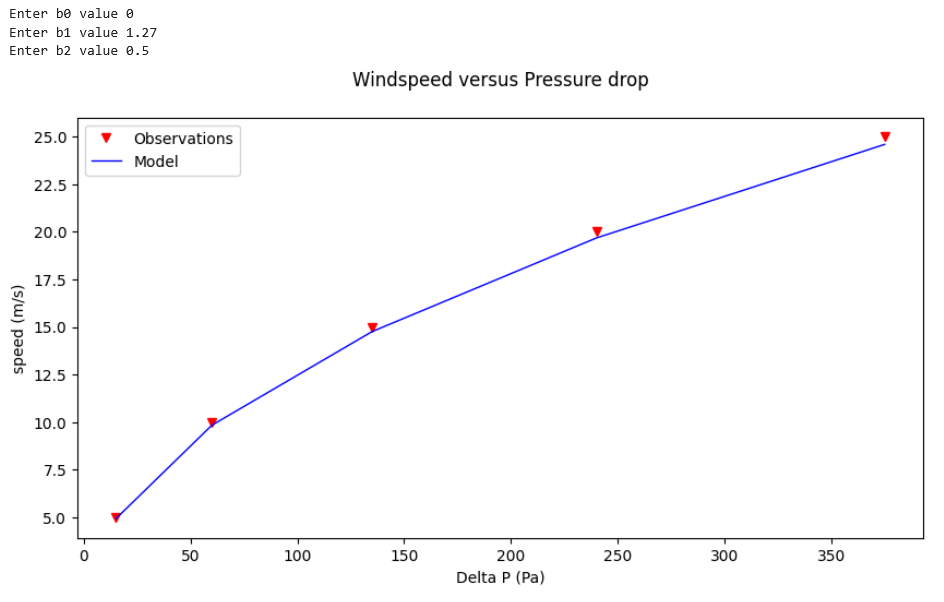
\includegraphics[height=4in]{Fitted.png} 
   \caption{Measured airspeed vs. Pressure Drop.  Markers are observations, line is fitted model (calculated airspeed using above equations).}
   \label{fig:pressure}
\end{figure}

The model used is\footnote{This model is identical to the Bernoulli equation representation.}
\begin{equation}
V_{mod}=0.0+1.27\times(\Delta P)^{0.5}
\end{equation}

\clearpage
\begin{enumerate}

\item Compare to Reference Velocity:
Compare the calculated airspeed from the Pitot tube with the wind tunnel’s reference airspeed. Plot a calibration curve of measured airspeed vs. reference airspeed.

\begin{figure}[h!] %  figure placement: here, top, bottom, or page
   \centering
   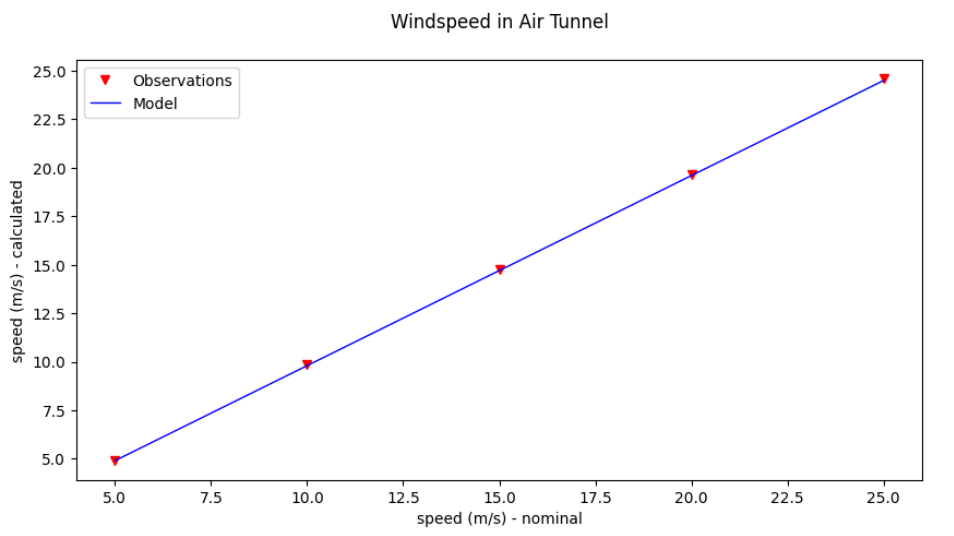
\includegraphics[height=4in]{Calibration.png} 
   \caption{Reference airspeed vs. Pitot airspeed.  Markers are observations, line is calibration curve.}
   \label{fig:windspeed}
\end{figure}

The model used is
\begin{equation}
V_{pitot}=0.0+0.98\times(V_{nominal})
\end{equation}

\item Calibration Curve: Use the data to create a plot (e.g., in Excel or Python) with the reference airspeed on the x-axis and the calculated airspeed on the y-axis. Ideally, the points should lie on the 1:1 line, but any deviations will indicate a correction factor for the Pitot tube calibration. Figure \ref{fig:windspeed} is a plot of nominal windspeed and Pitot tube airspeed - the solid line is the calibration curve.

\end{enumerate}
%%%%%%%%%%%%%%%%%%%%%%%%%%%%%
\clearpage

\section{Interpretation \& Engineering Judgment:} 
In this section, interpret your results:
\begin{itemize}
\item Compare the calculated airspeed values to the reference airspeeds from the wind tunnel.
\item Discuss any discrepancies between the two measurements. Were they consistent? Did the Pitot tube require calibration?
\item Discuss potential sources of error (e.g., alignment of the Pitot tube, calibration of the pressure transducer, or air density variations).
\end{itemize}
%%%%%%%%%%%%%%%%%%%%%%%%%%%%%
\clearpage

\section{Conclusions:} 
Bullet list of the 2–4 takeaways that answer the objective(s). Include recommended next steps.
\begin{itemize}
\item The calculated airspeed values are/are not consistent with the reference airspeeds from the wind tunnel.
\item Discuss potential sources of error (e.g., alignment of the Pitot tube, calibration of the pressure transducer, or air density variations).
\item Suggest improvements to the experimental setup or procedures that could reduce error in future experiments.
\end{itemize}
%%%%%%%%%%%%%%%%%%%%%%%%%%%%%
\clearpage

\begin{thebibliography}{}

\bibitem[Holman(2012)]{Holman2012}
Holman, J.P., 2012. Experimental Methods for Engineers, 8th Ed. 
\url{https://mech.at.ua/HolmanICS.pdf}

\bibitem[Gupta(2017)]{Gupta2017}
Gupta, R.S. 2017. Hydrology and Hydraulic Systems 4th ed. Waveland Press, Inc. ISBN 978-1-4786-3091-3 888p.

\bibitem[Cleveland(2024)]{Cleveland2024}
Cleveland, T. G. 2024. Engineering Hydrology Instructor's Notes and Selected Readings to accompany CE-3354, Department of Civil, Environmental, and Construction Engineering, Whitacre College of Engineering. \url{http://54.243.252.9/ce-3354-webroot/}

\end{thebibliography}
%%%%%%%%%%%%%%%%%%%%%%%%%%%%%
\clearpage

\section{Appendices}

\section*{Scripts to Generate Plots}
\begin{verbatim}
import matplotlib.pyplot as plt
def make2plot(listx1,listy1,listx2,listy2,strlablx,strlably,strtitle):
    mydata = plt.figure(figsize = (10,5)) # build a square drawing canvass from figure class
    plt.plot(listx1,listy1, c='red', marker='v',linewidth=0) # basic data plot
    plt.plot(listx2,listy2, c='blue',linewidth=1) # basic model plot
    plt.xlabel(strlablx)
    plt.ylabel(strlably)
    plt.legend(['Observations','Model'])# modify for argument insertion
    plt.title(strtitle)
    plt.show()
    return

def linear(b0,b1,x):
    ''' 
    linear data model, b0,b1 are parameters
    return y = b0+b1*x
    '''
    linear=b0+b1*x
    return(linear)

def quadratic(b0,b1,b2,x):
    ''' 
    quadratic data model, b0,b1 are parameters
    return y = b0+b1*x+b2*x^2
    '''
    quadratic=b0+b1*x+b2*x**2
    return(quadratic)  

def powerlaw(b0,b1,b2,x):
    '''
    power law data model
    return y = b0 + b1*x**b2'''
    powerlaw=b0+b1*x**b2
    return(powerlaw)

def residue(list1,list2,list3):
    ''' 
    compute residues
    list3 = list1 - list2
    return residuals in list3
    '''
    if len(list1)!=len(list2) or len(list1)!=len(list3):
        print('Lists unequal length, undefined operations')
        return
    for i in range(len(list1)):
        list3[i]=list1[i]-list2[i]
    return(list3)



ytable = [5,10,15,20,25] # nominal windspeed
xtable = [15,60,135,240,375] #pressure drop in pitot tube


# Fit a data model - power-law model
b0=float(input('Enter b0 value'))
b1=float(input('Enter b1 value'))
b2=float(input('Enter b2 value'))
# build a data model
modelYYY = [] # empty list
for i in range(len(xtable)):
    modelYYY.append(powerlaw(b0,b1,b2,xtable[i]))
# Plotting results
make2plot(xtable,ytable,xtable,modelYYY,'Delta P (Pa)','speed (m/s)','Windspeed versus Pressure drop\n ')

# build a data model
modelZZZ = [] # empty list
for i in range(len(ytable)):
    modelZZZ.append(linear(0,0.98,ytable[i])) # fitted velocity pitot vs velocity nominal
make2plot(ytable,modelYYY,ytable,modelZZZ,'speed (m/s) - nominal','speed (m/s) - calculated','Windspeed in Air Tunnel\n ')

\end{verbatim}


\end{document}  